\subsection{\label{sec:calib.tag}Tagger Timing Calibration}
The timing calibration of the tagger system was performed using the standard procedures. Overall, the quality of the calibration is excellent, showing an overall timing resolution of about $130$~ps, when the tagger time is compared with the RF time. The counter-by-counter alignment can be seen on Fig.~\ref{tagtpho}. The calibration was checked on a run by run basis (Fig.~\ref{tagRun}), and new constants were commissioned when major changes were noticed.

Notice the steps in resolution for the tagger timing is 160 ps before about run 56650 and 130 ps afterwards. This is due to a change in the production trigger, which shifted trigger preference to higher energy photons. The high energy T-counters have better resolutions which explains this shift.


\begin{figure}[htpb]
\begin{center}
 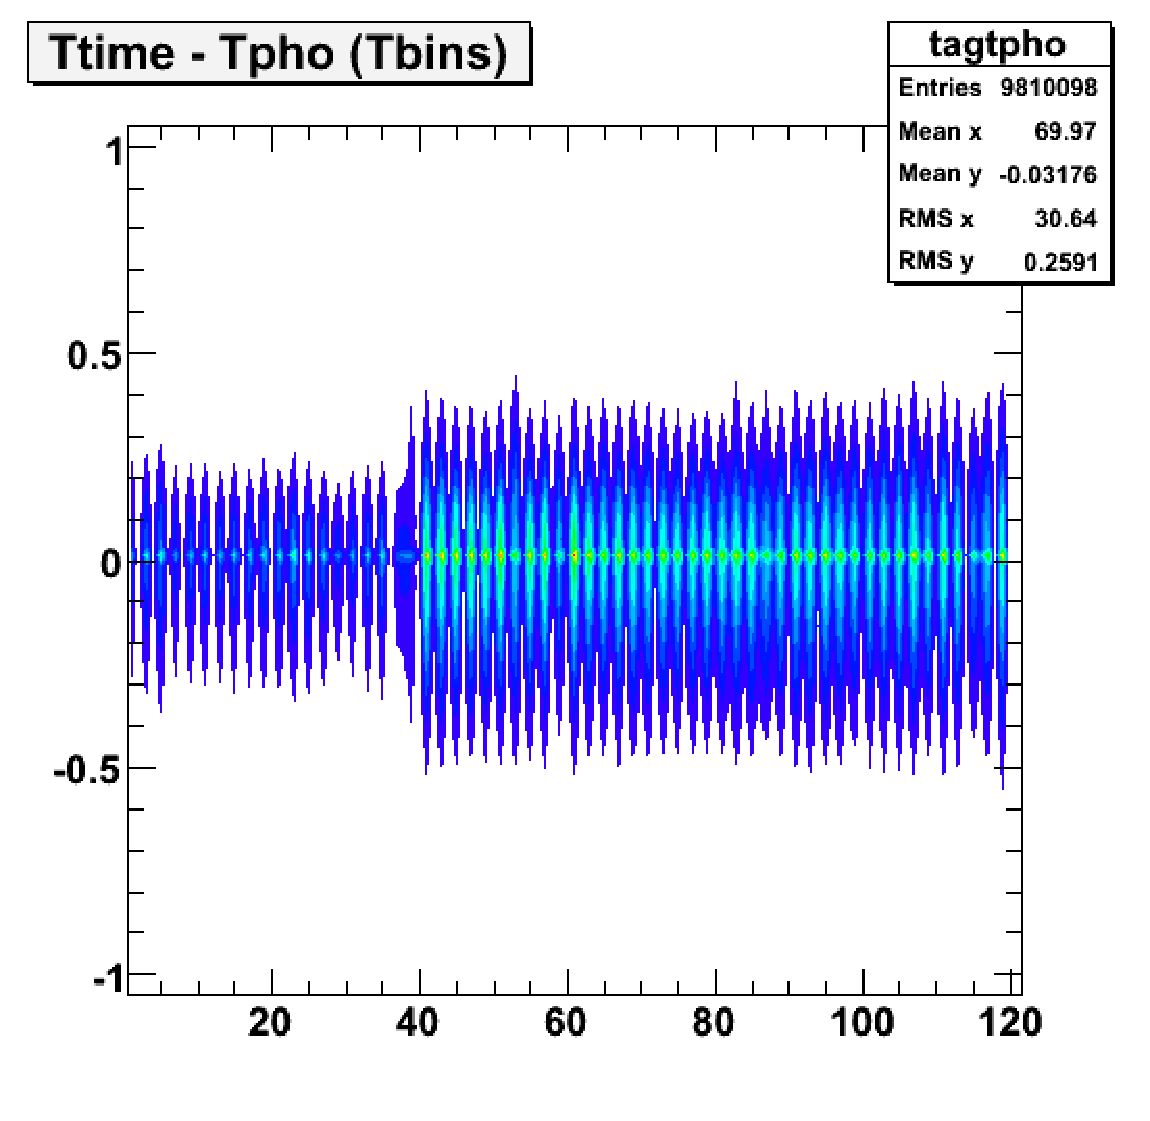
\includegraphics[width=0.45\textwidth]{figures/calib/tag/timing/tagtpho.eps}
  \caption{And example of the tagger timing calibration and the T-counter alignment, comparing  the difference between photon time determined from the tagger elements (T-counters, in this particular plot), and photon timing according to the RF. The relative intensity of the paddles shown are due to the trigger configuration, see Tables.~\ref{tab:data.trig.conf.2} and \ref{tab:data.trig.mor}.}
  \label{tagtpho}
  \end{center}
\end{figure}


\begin{figure}[htpb]
\begin{center}
 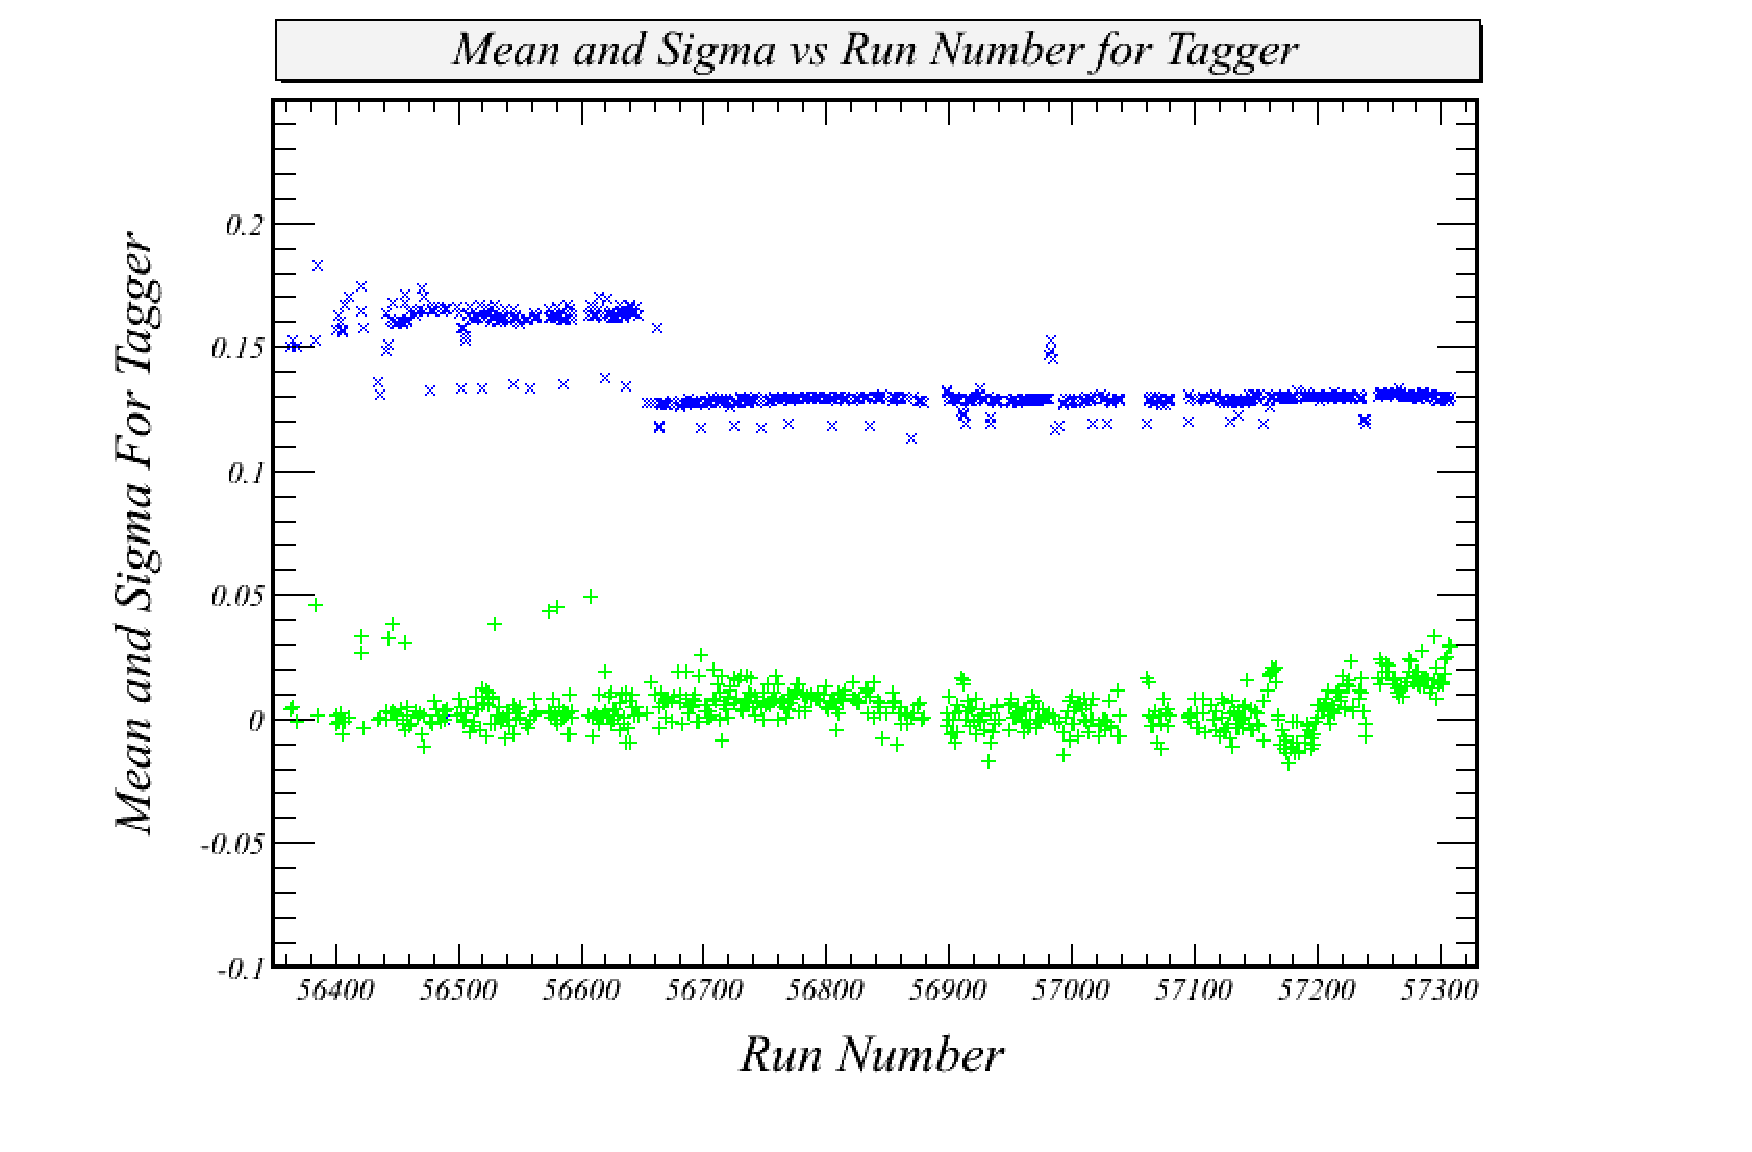
\includegraphics[width=0.45\textwidth]{figures/calib/tag/timing/tagRun.eps}
  \caption{The run-by-run behavior of the tagger timing calibration where the mean is in green and the sigma is in blue. Overall, the tagger timing resolution is about $130$~ps for the production runs, and the mean behaves stably throughout the running period.}
  \label{tagRun}
  \end{center}
\end{figure}
